\documentclass[11pt]{article}
\usepackage[a4paper, total={6.8in, 9.25in}]{geometry}
\usepackage{graphicx}
\graphicspath{ {./assets/images/output/} }
\usepackage{caption}
\usepackage[english]{babel}
\usepackage{titling}
\usepackage{float}
\usepackage{amsmath}
\usepackage{algorithm}
\usepackage{algorithmicx}
\usepackage{algpseudocode}
\usepackage{minted}
\usepackage{multicol}
\usepackage{array}
\usepackage{setspace}
\usepackage{placeins}
\usepackage{tcolorbox}
\usepackage{caption}
\usepackage{subcaption}

\definecolor{verbgray}{gray}{.95}
\setminted{
    bgcolor=verbgray,
    baselinestretch=1,
    fontsize=\footnotesize,
    linenos,
    breaklines=true,
    breakanywhere=true,
    xleftmargin=\parindent
}
\title{Implementation \& Evaluation of Single Layer Perceptron (SLP) and Multi-Layer Perceptron (MLP)}
\author{}
\date{}

\pagenumbering{gobble}
\begin{document}
\input{ml_cover.tex}

\pagebreak

\tableofcontents

\pagebreak
\pagenumbering{arabic}
\maketitle

\section{Theory and Introduction}
Artificial Neural Networks (ANNs) are computational models inspired by the human brain. This experiment explores the fundamental building blocks of ANNs by implementing a Single Layer Perceptron (SLP) and a Multi-Layer Perceptron (MLP) from scratch to evaluate their capabilities on linear and non-linear classification tasks.

\subsection{Single Layer Perceptron (SLP)}
The Single Layer Perceptron is the simplest form of a neural network, consisting of a single layer of output nodes connected directly to a layer of inputs. It is a linear binary classifier \cite{bishop2006pattern}.

\subsubsection*{Hypothesis and Activation}
The SLP computes a linear combination of inputs $x$ and weights $w$, adding a bias $b$:
\begin{equation}
    z = \sum_{i=1}^{n} w_i x_i + b = w^T x + b
\end{equation}
A step function is then applied to act as the activation function, squashing the output to a binary class ($0$ or $1$):
\begin{equation}
    f(z) =
    \begin{cases}
        1 & \text{if } z \geq 0 \\
        0 & \text{otherwise}
    \end{cases}
\end{equation}

\subsubsection*{Weight Update Rule}
The perceptron updates its weights based on the prediction error $e = (y - \hat{y})$. If the prediction is correct, no update occurs. Otherwise, the weights are adjusted iteratively:
\begin{equation}
    w_i \gets w_i + \alpha (y - \hat{y}) x_i
\end{equation}
where $\alpha$ is the learning rate.

\subsection{Multi-Layer Perceptron (MLP)}
An MLP introduces one or more hidden layers between the input and output layers. This architecture, coupled with non-linear activation functions, allows the network to learn complex, non-linear decision boundaries \cite{goodfellow2016deep}.

\subsubsection*{Forward Propagation}
For a network with one hidden layer, the forward pass involves computing the linear combinations and applying the Sigmoid activation function $\sigma(z) = \frac{1}{1 + e^{-z}}$ sequentially:
\begin{equation}
    A^{[1]} = \sigma(W^{[1]} X + b^{[1]}) \quad \text{(Hidden Layer)}
\end{equation}
\begin{equation}
    A^{[2]} = \sigma(W^{[2]} A^{[1]} + b^{[2]}) \quad \text{(Output Layer)}
\end{equation}

\subsubsection*{Cost Function and Backpropagation}
The MLP minimizes the Binary Cross-Entropy (Log Loss) function over $m$ samples:
\begin{equation}
    J = -\frac{1}{m} \sum_{i=1}^{m} \left[ y^{(i)} \log(A^{[2](i)}) + (1 - y^{(i)}) \log(1 - A^{[2](i)}) \right]
\end{equation}
Weights are updated using the Backpropagation algorithm, which computes the gradients of the cost function with respect to the network parameters using the chain rule.

\section{Methodology}

\subsection{Datasets}
Two datasets were utilized to demonstrate the capabilities and limitations of each network:
\begin{itemize}
    \item \textbf{California Housing (SLP):} A linear classification task created by converting median house values into binary classes ("Low Value" vs "High Value").
    \item \textbf{Two Moons (MLP):} A synthetic dataset consisting of two interleaving half circles, serving as a classic non-linear classification benchmark.
\end{itemize}

\subsection{Algorithms}

\begin{algorithm}[H]
    \caption{Single Layer Perceptron (Training Phase)}
    \begin{algorithmic}[1]
        \State \textbf{Initialize} weights $W \gets 0$, bias $b \gets 0$
        \For{$epoch = 1$ to $N$}
        \For{each sample $(x_i, y_i)$}
        \State $z \gets W^T x_i + b$
        \State $\hat{y} \gets 1 \text{ if } z \geq 0 \text{ else } 0$
        \State $update \gets \alpha (y_i - \hat{y})$
        \State $W \gets W + update \cdot x_i$
        \State $b \gets b + update$
        \EndFor
        \EndFor
    \end{algorithmic}
\end{algorithm}

\begin{algorithm}[H]
    \caption{Multi-Layer Perceptron (Forward \& Backward Prop)}
    \begin{algorithmic}[1]
        \State \textbf{Initialize} $W^{[1]}, b^{[1]}, W^{[2]}, b^{[2]}$ randomly
        \For{$epoch = 1$ to $N$}
        \State $A^{[1]} \gets \sigma(W^{[1]} X + b^{[1]})$ \Comment{Forward Pass}
        \State $A^{[2]} \gets \sigma(W^{[2]} A^{[1]} + b^{[2]})$
        \State $Cost \gets \text{LogLoss}(A^{[2]}, Y)$
        \State $dZ^{[2]} \gets A^{[2]} - Y$ \Comment{Backward Pass}
        \State $dW^{[2]} \gets \frac{1}{m} A^{[1]T} dZ^{[2]}$
        \State $dZ^{[1]} \gets (dZ^{[2]} W^{[2]T}) * A^{[1]}(1 - A^{[1]})$
        \State $dW^{[1]} \gets \frac{1}{m} X^T dZ^{[1]}$
        \State \textbf{Update} Parameters using gradients and learning rate $\alpha$
        \EndFor
    \end{algorithmic}
\end{algorithm}

\subsection{Code Implementation}
The networks were implemented natively using Python and NumPy.
\subsubsection*{SLP}
\begin{multicols}{2}
    \inputminted{Python}{./assets/slp.py}
\end{multicols}

\subsubsection*{MLP}
\begin{multicols}{2}
    \inputminted{Python}{./assets/mlp.py}
\end{multicols}

\section{Results and Discussion}

\subsection{Single Layer Perceptron (Linear Classification)}
The SLP was tested on the California Housing binary classification task. Since the dataset is not perfectly linearly separable, the errors per epoch fluctuated rather than dropping to absolute zero.

\begin{minted}{console}
 SINGLE LAYER PERCEPTRON (SLP) CLASSIFICATION

Loading California Housing Dataset...
Dataset Shape: (2000, 8)
Target distribution: [ 999 1001]

Training Perceptron...
========================================
EVALUATION REPORT
========================================
Accuracy:  0.7825
Precision: 0.8508
Recall:    0.7196
F1 Score:  0.7797
Confusion Matrix:
[[159  27]
 [ 60 154]]
\end{minted}

The SLP achieved an accuracy of 78.25\%. Figure \ref{fig:slp_results} illustrates the convergence behavior and the learned decision boundary. The straight boundary confirms that the SLP can only isolate linearly separable regions, contributing to the instances of false positives and false negatives seen in the confusion matrix.

\begin{figure}[H]
    \centering
    \begin{subfigure}[b]{0.45\textwidth}
        \centering
        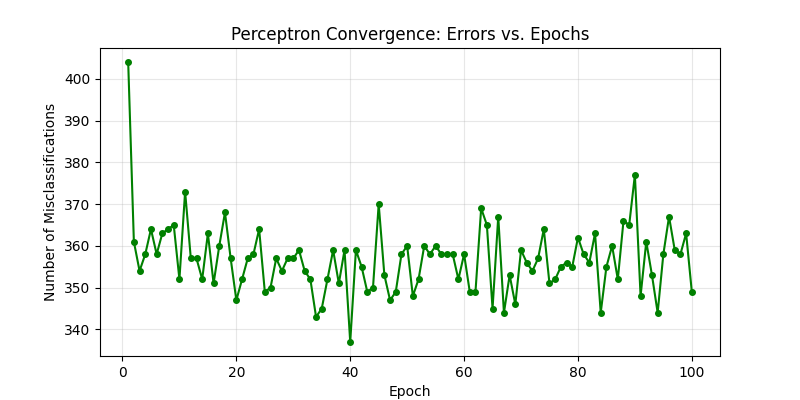
\includegraphics[width=\textwidth]{slp_errors_history.png}
        \caption{Errors per Epoch}
    \end{subfigure}
    \hfill
    \begin{subfigure}[b]{0.45\textwidth}
        \centering
        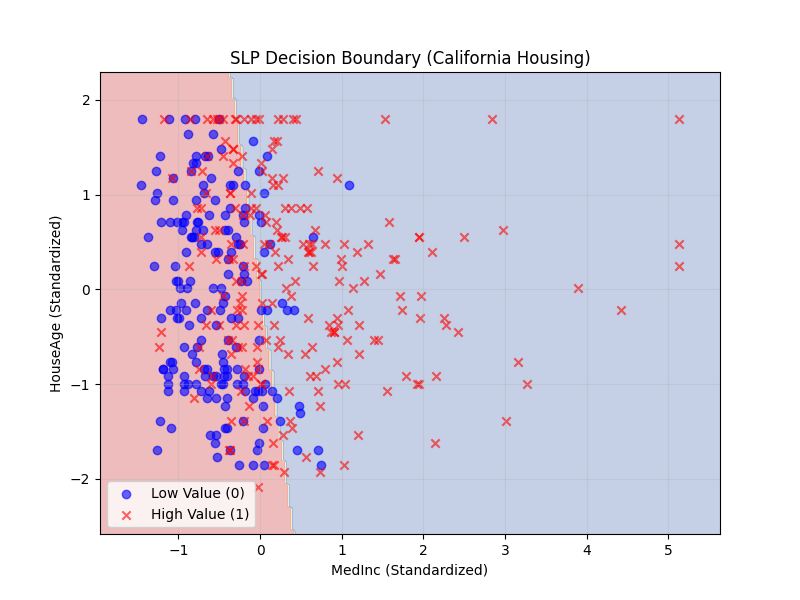
\includegraphics[width=\textwidth]{slp_decision_boundary.png}
        \caption{Linear Decision Boundary}
    \end{subfigure}

    \vspace{0.5cm}
    \begin{subfigure}[b]{0.4\textwidth}
        \centering
        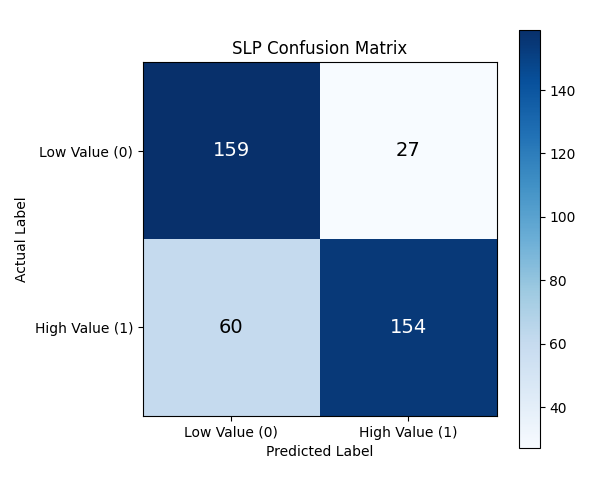
\includegraphics[width=\textwidth]{slp_conf_matrix.png}
        \caption{Confusion Matrix}
    \end{subfigure}
    \caption{Single Layer Perceptron Performance Overview}
    \label{fig:slp_results}
\end{figure}

\subsection{Multi-Layer Perceptron (Non-Linear Classification)}
The MLP (architecture: 2 inputs $\to$ 4 hidden neurons $\to$ 1 output) was trained on the non-linear "Two Moons" dataset.

\begin{minted}{console}
 MULTI-LAYER PERCEPTRON (NON-LINEAR CLASSIFICATION)
Generating 'Two Moons' dataset...

Training MLP (2 Inputs -> 4 Hidden -> 1 Output) on 800 samples...
Epoch 0 | Cost: 0.6933
Epoch 1000 | Cost: 0.2808
Epoch 2000 | Cost: 0.2761
Epoch 3000 | Cost: 0.2741
Epoch 4000 | Cost: 0.2730
========================================
EVALUATION REPORT
========================================
Accuracy:  0.8600
Precision: 0.8600
Recall:    0.8600
F1 Score:  0.8600
Confusion Matrix:
[[86 14]
 [14 86]]
\end{minted}

The MLP achieved a balanced accuracy, precision, and recall of 86.00\%. The cost history demonstrates a smooth convergence, indicating successful backpropagation. Figure \ref{fig:mlp_results} visually highlights the MLP's ability to bend the decision boundary through the hidden layer transformations, successfully separating the crescent shapes that an SLP would fail to capture.

\begin{figure}[H]
    \centering
    \begin{subfigure}[b]{0.4\textwidth}
        \centering
        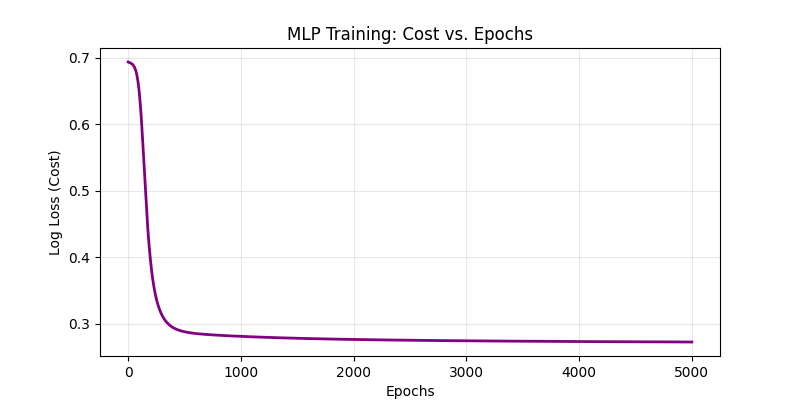
\includegraphics[width=\textwidth]{mlp_cost_history.png}
        \caption{Cost (Log Loss) vs. Epochs}
    \end{subfigure}
    \hfill
    \begin{subfigure}[b]{0.36\textwidth}
        \centering
        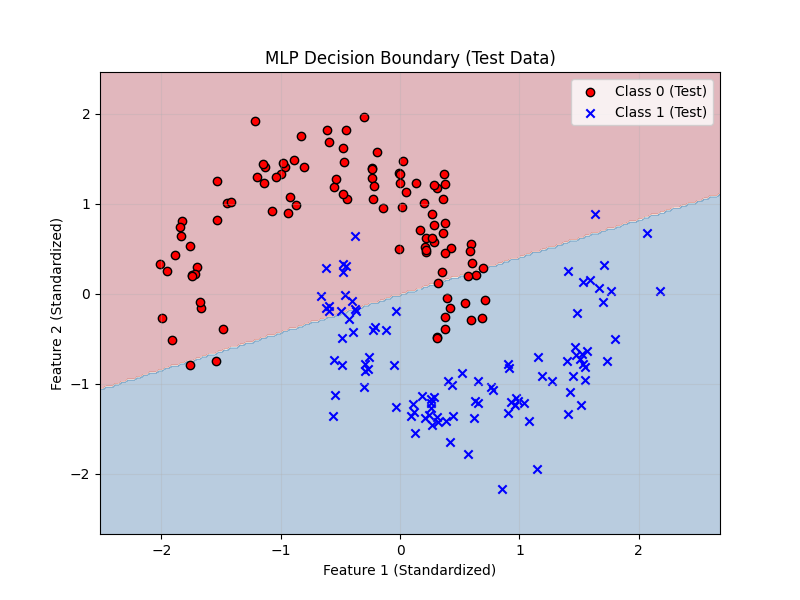
\includegraphics[width=\textwidth]{mlp_decision_boundary.png}
        \caption{Non-Linear Decision Boundary}
    \end{subfigure}

    \vspace{0.5cm}
    \begin{subfigure}[b]{0.3\textwidth}
        \centering
        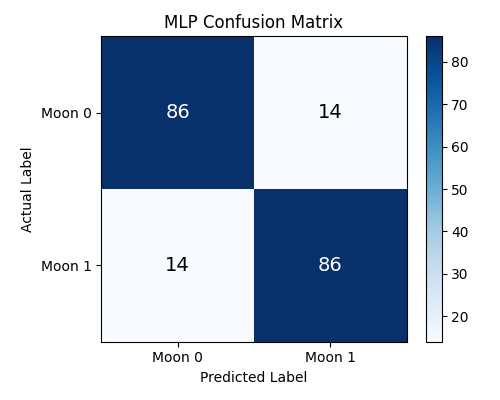
\includegraphics[width=\textwidth]{mlp_conf_matrix.png}
        \caption{Confusion Matrix}
    \end{subfigure}
    \caption{Multi-Layer Perceptron Performance Overview}
    \label{fig:mlp_results}
\end{figure}

\section{Conclusion}
This experiment successfully demonstrated the distinction between linear and non-linear classification models.
\begin{itemize}
    \item The \textbf{Single Layer Perceptron} is highly efficient but structurally limited to linearly separable datasets. Its failure to converge perfectly on real-world housing data illustrates the limitation of single-layer architectures.
    \item The \textbf{Multi-Layer Perceptron} overcomes these limitations. By introducing hidden neurons and non-linear Sigmoid activations, it successfully maps complex geometric boundaries, as proven by its strong performance on the Two Moons dataset.
\end{itemize}

\bibliographystyle{IEEEtran}
\renewcommand{\bibname}{References}
\addcontentsline{toc}{section}{References}
\bibliography{ref}

\end{document}